% !TeX spellcheck = en_GB
\chapter{Analysis}
\epigraph{Without requirements or design, programming is the art\\of adding bugs to an empty text file.}{Louis Srygley}
\section{Terminology}
Taking into account that the intended audience for this thesis are developers and operators of security reporting systems, 
we mostly use the  Security Automation and Continuous Monitoring (SACM) terminology~\cite{ietf-sacm-terminology-14}
and thereby follow the same guidelines as the XMPP grid draft~\cite{ietf-mile-xmpp-grid-05}.

\section{Technical Background}\label{sec:technical-background}

The following sections introduce the underlying XMPP protocol and the relevant extensions (\glspl{xep}) used by the XMPP grid draft as well as a summary of it and the corresponding XMPP terminology.

\subsection{XMPP (eXtensible Messaging and Presence Protocol)}
The Extensible Messaging and Presence Protocol (in short \gls{xmpp}) is an open protocol that enables the near-real-time exchange of small data between any network endpoints, hereafter called \glspl{platform}~\cite{rfc6120}.
While originally designed as an Instant Messaging (IM) protocol, XMPP can be used for a wide range of data exchange applications~\cite{ieee-xplore-stream-xml-xmpp}.

XMPP is made of small building blocks defined in the core protocol~\cite{rfc6120} and numerous extensions called \glspl{xep}~\cite{xep-0001}.
The core is comprised of functionality for setup and encryption of communication channels, \gls{xml} streams, error handling and more. Additional functionality such as \gls{service-discovery}~\cite{xep-0030} and \gls{publish-subscribe}~\cite{xep-0060} are defined in separate extensions.

Although XMPP supports peer-to-peer communication, it is often used in a traditional client-server architecture.
A client (\gls{platform}) can send data to any addressable entity (any other \glspl{platform}) using \Gls{jabber} Identifiers, hereafter called \gls{jid}. If the \gls{jid} of the receiver has a different domainpart than the current server (\gls{controller}), the message is forwarded to the responsible XMPP server under its domain~\cite{rfc6120}.

The data exchanged over XMPP is \gls{xml} which makes the protocol structured and extensible, but leads to some protocol overhead.
XMPP communicates over unidirectional data streams with a server, which are basically long-lived \gls{tcp} connections.
The client opens a channel to the server over this connection, and the server opens one back (i.e. \code{<stream>} XML tags). In both streams, an XML document is opened after the connection is established.
During the conversation, an arbitrary amount of \glspl{stanza} (specified XML child elements) are written to the stream.
Before a connection may be terminated, the root element is closed (i.e. \code{</stream>}) and both streams form valid XML documents~\cite{rfc6120}\cite{professional-xmpp}.

The core \gls{stanza} types are \glspl{message}~(\code{<message/>}), \gls{presence}~(\code{<presence/>}) and\\
\gls{info-query}~(\code{<iq/>}).
\Glspl{message} can contain arbitrary data similar to email but are optimised for immediate delivery.
\Gls{presence} \glspl{stanza} deal with network availability and the propagation of user presence information.
An \gls{info-query} \gls{stanza} consists of a request and response (similar to the GET and POST HTTP methods), which is used for feature negotiation, configuration and general information exchange.
Because of these coarse semantics, XMPP provides a generalized communication layer~\cite{rfc6120}\cite{ieee-xplore-stream-xml-xmpp}.

Figure~\ref{fig:xmpp-overview} illustrates an example setup with two servers and three clients.

\begin{figure}[h]
	\centering
	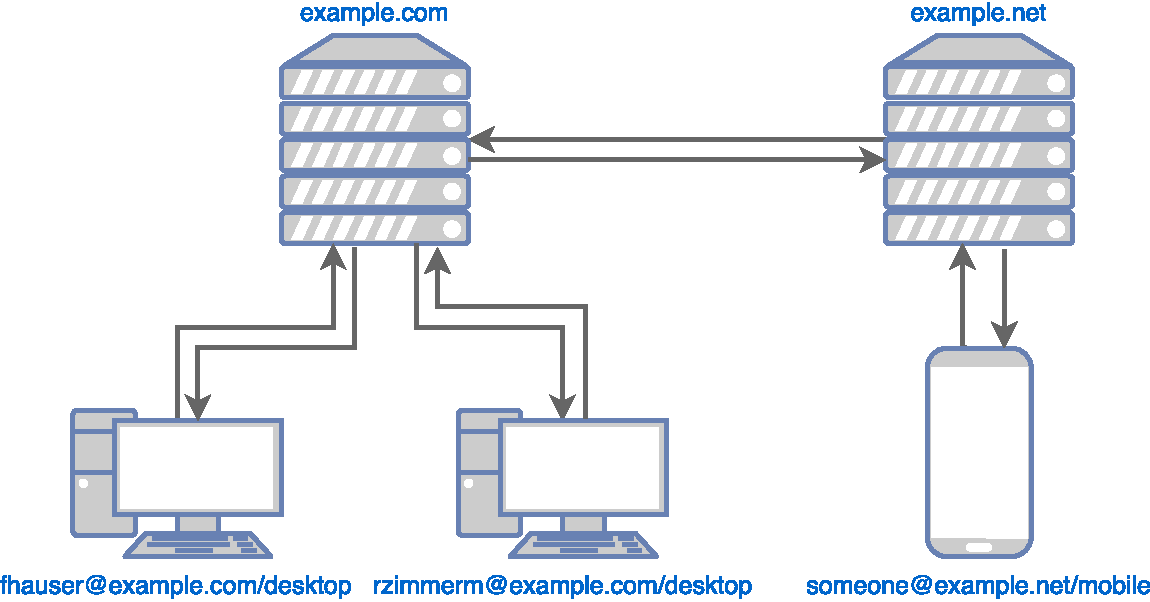
\includegraphics[width=0.8\linewidth]{resources/xmpp_overview.pdf}
	\caption{Two XMPP domains (servers), one with two users and one with a single mobile user.}
	\label{fig:xmpp-overview}
\end{figure}

\subsection{Relevant XMPP Extensions}

The XMPP grid draft~\cite{ietf-mile-xmpp-grid-05} is based on multiple \glspl{xep}, most notably \gls{publish-subscribe}. In this section, we give an overview of the most relevant used \glspl{xep}.

\paragraph{XEP-0004: \gls{data-forms}} is a flexible protocol that can be used in workflows such as service configuration as well as for application-specific data description and reporting. The protocol provides form processing, common field types and extensibility mechanisms~\cite{xep-0004}.

\paragraph{XEP-0030: \gls{service-discovery}} enables entities to discover information about the identity and capabilities of other entities, e.g. whether the entity is a server or not, or items associated with an entity, e.g. a list of \gls{publish-subscribe} nodes~\cite{xep-0030}.

\paragraph{XEP-0059: \Gls{result-set-management}} allows entities to manage the receipt of large result sets, e.g. by paging through the result or limiting the number of results. \gls{result-set-management} is often desired when dealing with large dynamic result sets, as from service discovery or publish-subscribe, and time or other resources are limited~\cite{xep-0059}.

\subsubsection{XEP-0060: \Gls{publish-subscribe}}
The \gls{publish-subscribe} Extension, hereafter referred to as \gls{pubsub} or \gls{broker}, enables XMPP entities (\gls{provider}) to broadcast information via \glspl{topic} to subscribed entities (\gls{consumer})~\cite{xep-0060}.

Nodes, hereafter referred to as \glspl{topic}, are the communication hubs. Entities can create topics and configure them, e.g. set up subscription timeouts or limit publishing and subscription rights. The configuration mechanism is based on data forms (XEP\babelhyphen{nobreak}0004). An XMPP-Server \emph{may} restrict node creation to certain entities, which means that possibly not every XMPP-Server that supports \gls{publish-subscribe} also implements this feature \cite{rfc2119}.

The protocol defines a hierarchy of six affiliations of which only the implementation of `owner` and `none` is \emph{required}.
The implementation of the remaining four affiliations is \emph{recommended}.
An owner of a topic can manage the subscriptions and affiliations of other entities associated with a given topic.

To simplify the creation of topics, \gls{pubsub} defines five topic access models ("node access models") that \emph{should} be available: open, presence, roaster, authorize and whitelist.

The open model allows uncontrolled access while presence and roaster are specific for IM. Using the authorize model, the owner has to approve all subscription requests. The whitelist model enables the owner to maintain a list of entities that are allowed to subscribe.

\section{Requirements Analysis}
% NFR, priorisierung, Testbarkeit, Accessibility
% Anforderungen abgenommen?

We collected the functional requirements in the form of user stories.
User Stories are an established and widespread concept for describing and managing requirements in agile software projects.
In comparison to traditional tools for requirement analysis, user stories are more blured, leaving more space for changes. \cite{wirdemann2017scrum}

We created some separate user stories for non-functional requirements.
Additional non-functional requirements can be added during the project in the form of constraints. \cite{wirdemann2017scrum}

In the early phase of the project, we collected an initial set of user stories based on the task description and discussions with Prof.\ Dr.\ Steffen.
This initial set covered the creation and deletion of topics as well as  granting publish and subscribe privileges.
All user stories are listed in Appendix~\fullref{sec:requirements}.

After coarse prioritisation, Prof.\ Dr.\ Steffen approved the initial set of user stories that then served as the basis for the architectural concept draft.

Detailed implementation prioritisation of the user stories are carried out before every sprint in agreement with Prof.\ Dr.\ Steffen.

\section{Domain Analysis}

\subsection{IETF Internet-Draft: Using XMPP for Security Information Exchange}\label{sec:ietf-internet-draft-using-xmpp-for-security-information-exchange}
This IETF Internet draft describes how the XMPP protocol enhanced with the in Section~\ref{sec:technical-background} discussed XEPs, most notably the \gls{pubsub} extension, can be used for the exchange and distribution of security-relevant information between network devices. The draft assumes use of the Incident Object Description Exchange Format (IODEF)~\cite{rfc7970}.

One of the primary motivation for using XMPP for this task is the fast propagation of such security-relevant data.
Using XMPP for such a task also comes with its downsides. Most notably, because the XMPP server (\gls{broker}/\gls{controller}) is the central configuration component in charge of managing access permission, its compromisation has serious consequences.

The draft describes a trust model, thread model as well as specific countermeasures, e.g. to use at least TLS 1.2. These countermeasures also define restrictions of the XMPP protocol and its extensions, e.g. by limiting the topic access models of \gls{pubsub} to whitelist and authorized only~\cite{ietf-mile-xmpp-grid-05}.

\subsubsection{Information Exchange in the IODEF}

The XMPP Grid draft states that ``although [the exchanged] information can take the form of any structured data (XML, JSON, etc.), this document illustrates the principles of XMPP-Grid with examples that use the Incident Object Description Exchange Format (IODEF)''~\cite{ietf-mile-xmpp-grid-05}.

As IODEF is not strictly defined nor explicitly recommended by the XMPP Grid draft, the implementation of this protocol is not in the scope of this thesis.

\subsection{Domain Specific Language}

Figure~\ref{fig:architecturedslgriddraft} and \ref{fig:architecturedslxeps} present an overview of the relevant interactions and relationships between the different components as specified in the XMPP grid draft~\cite{ietf-mile-xmpp-grid-05} and as used in the referenced XEPs (see Section~\ref{sec:technical-background}).

\begin{figure}[h]
\centering
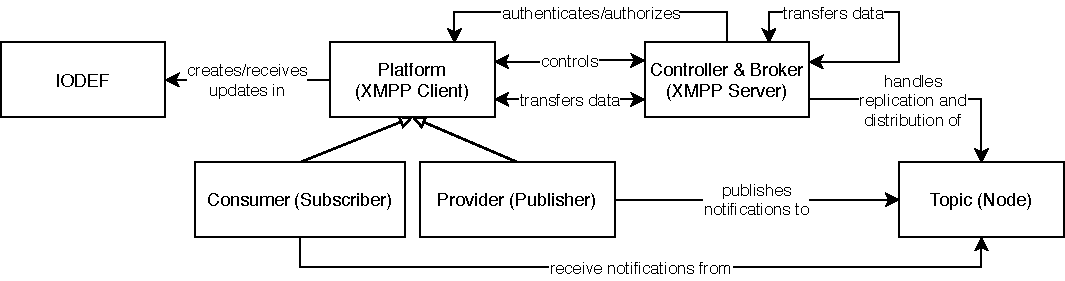
\includegraphics[width=\linewidth]{resources/architecture_dsl_grid_draft}
\caption[DSL of XMPP grid draft]{Domain Specific Language of the XMPP grid draft}
\label{fig:architecturedslgriddraft}
\end{figure}

\begin{figure}[h]
\centering
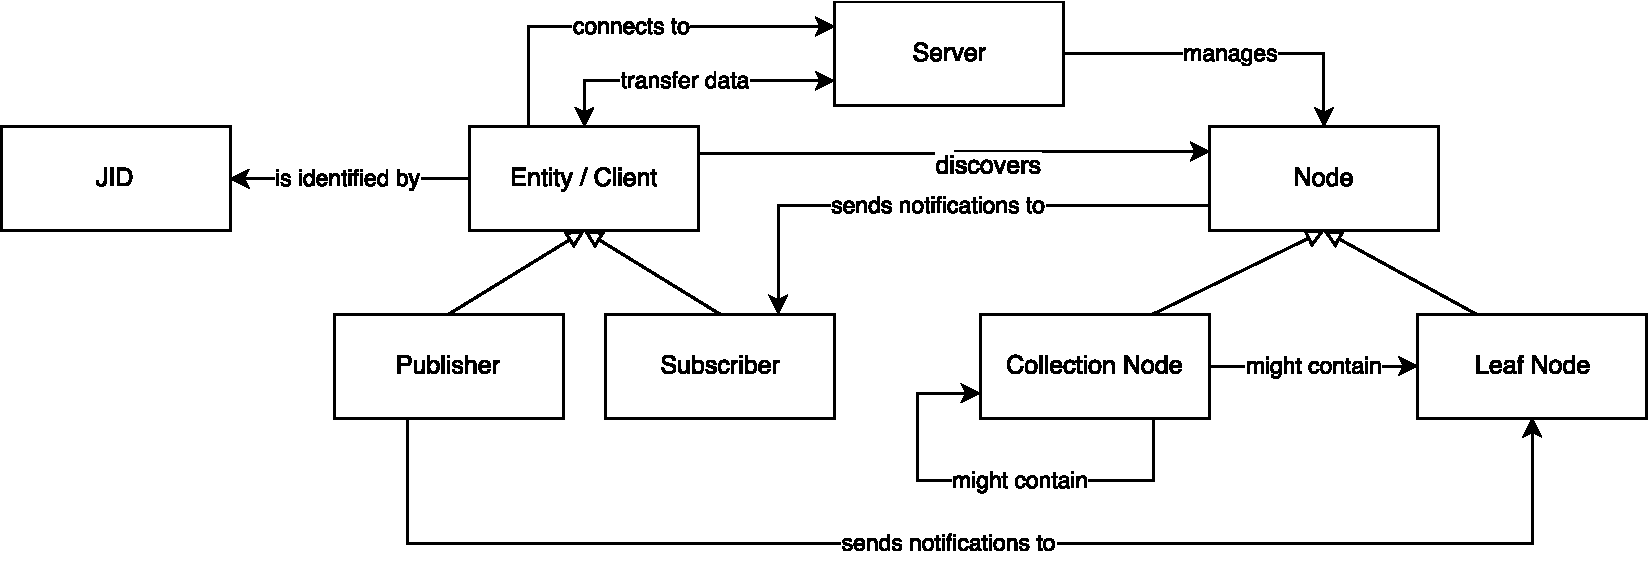
\includegraphics[width=\linewidth]{resources/architecture_dsl_xeps}
\caption[DSL of used XMPP XEPs]{Domain Specific Language of used XMPP XEPs}
\label{fig:architecturedslxeps}
\end{figure}


\section{Risk Analysis}
